\section{数据下载}
\subsection{获取链接}
\begin{frame}
    回到我们的订单内容页面
    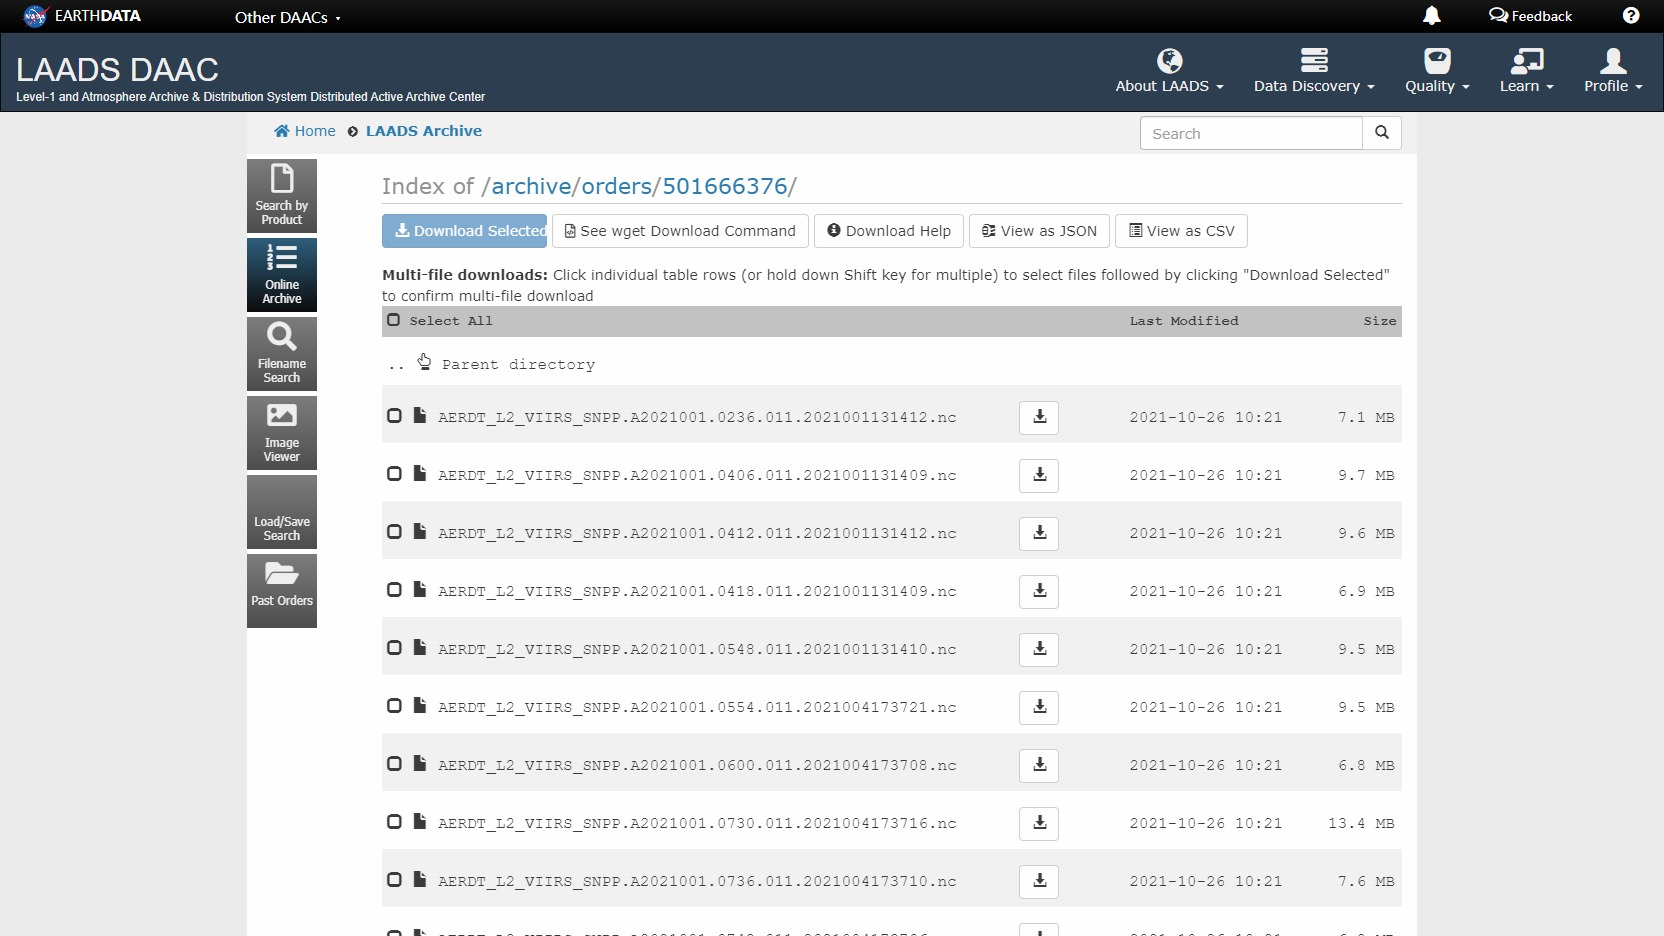
\includegraphics[width=\linewidth]{images/20.订单内容}
\end{frame}
\begin{frame}
    \frametitle{选中全部订单文件}
    点击\underline{Select All}复选框,选中全部文件
    \begin{annotationimage}{width=\linewidth}{images/20.订单内容}
        \draw[red,very thick](0.23,0.64) rectangle (0.3,0.68);
    \end{annotationimage}
\end{frame}
\begin{frame}[label=file-link]
    \frametitle{获取选中文件地址}
    点击\underline{Download All}按钮,获取选中文件的存储链地址
    \begin{annotationimage}{width=\linewidth}{images/24.全选订单文件}
        \draw[red,very thick](0.23,0.73) rectangle (0.33,0.77);
    \end{annotationimage}
\end{frame}
\begin{frame}
    \frametitle{全选文件地址}
    使用鼠标选中所有文件地址并复制\\
    但这不是可以直接下载的地址,所以请继续下一步
    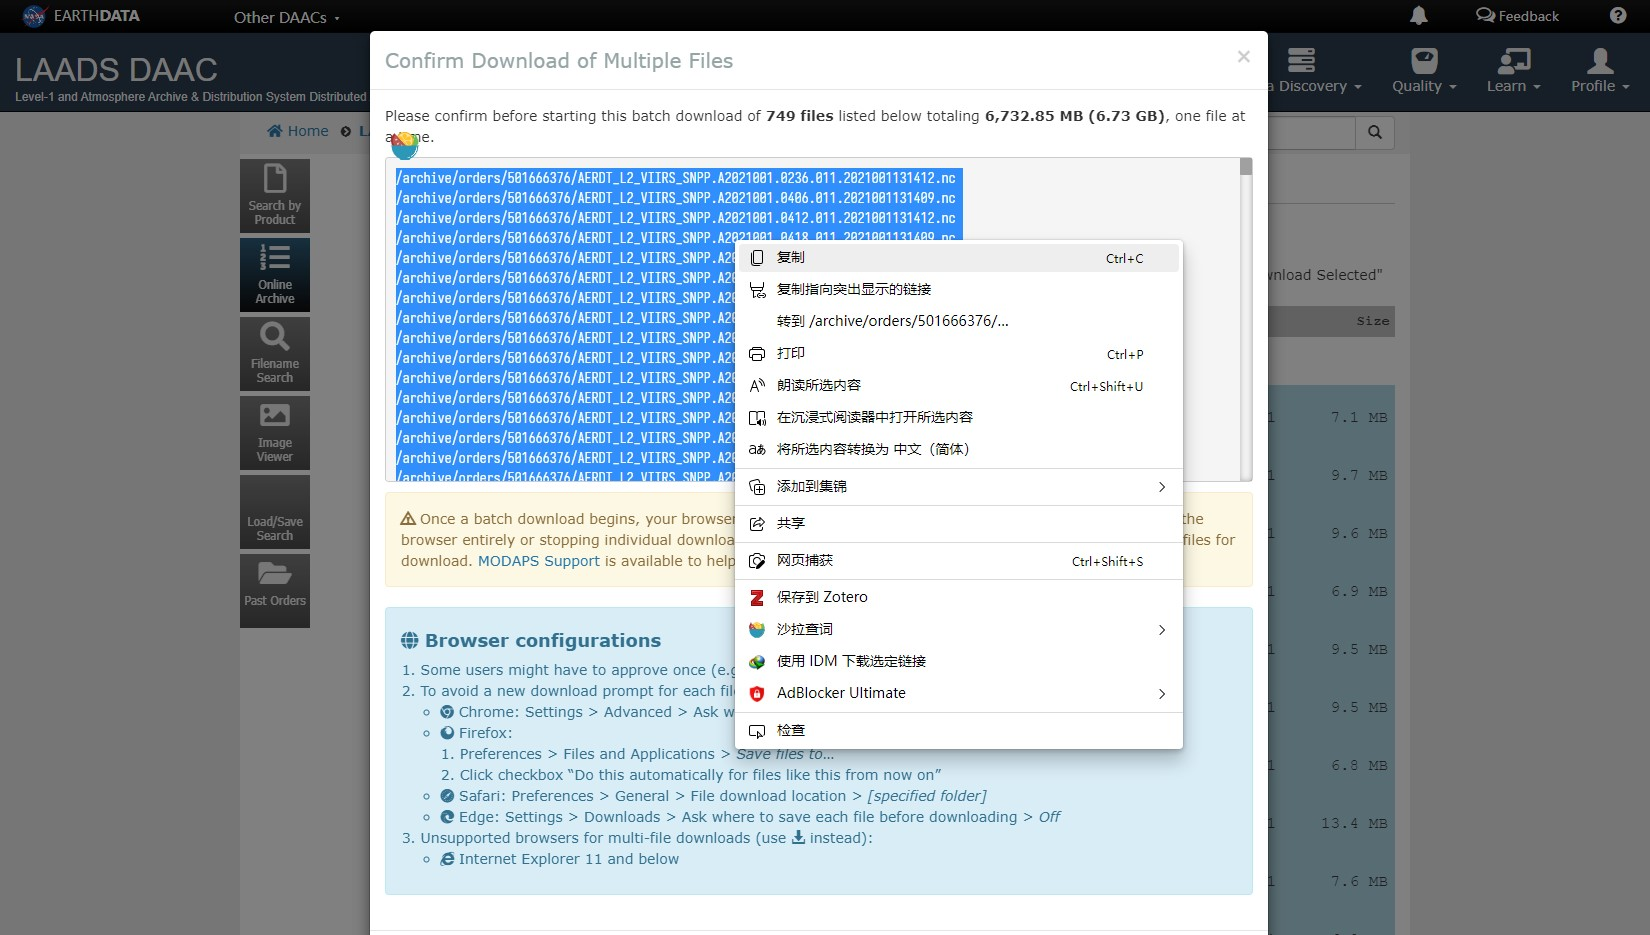
\includegraphics[width=\linewidth]{images/25.全选文件地址}
\end{frame}
\begin{frame}
    \frametitle{建立一个文件夹}
    找个清楚的地方新建一个文件夹,用来存放待下载的文件\\
    假如叫laads\_order\_501666376
    \begin{annotationimage}{width=\linewidth}{images/26.新建一个文件夹}
        \imagelabelset{image label back = white,image label text = black}
        \draw[image label = {501666376是该订单的订单号 at center}];
    \end{annotationimage}
\end{frame}
\begin{frame}
    \frametitle{存储文件地址}
    在该文件夹下新建一个文本文件,假如叫file\_download\_link.txt,将刚才复制的文件地址粘贴进来
    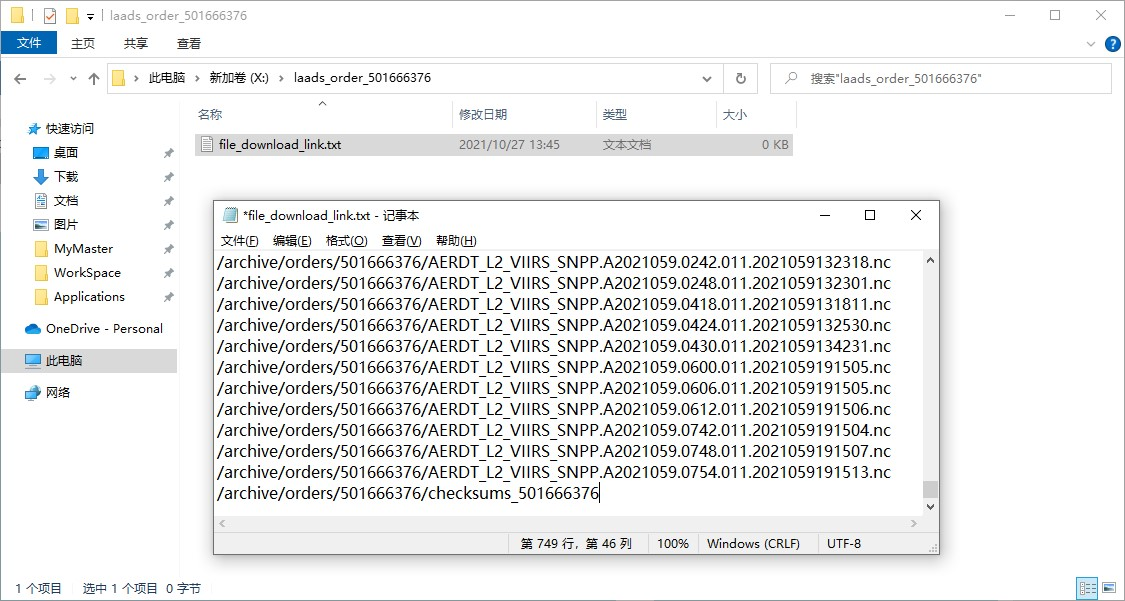
\includegraphics[width=\linewidth]{images/27.粘贴下载链接}
\end{frame}
\begin{frame}
    \frametitle{使用替换工具完善文件地址}
    在每个文件地址的开头加上https://ladsweb.modaps.eosdis.nasa.gov即为其真正的下载
    地址,我们使用替换工具实现这一目的
    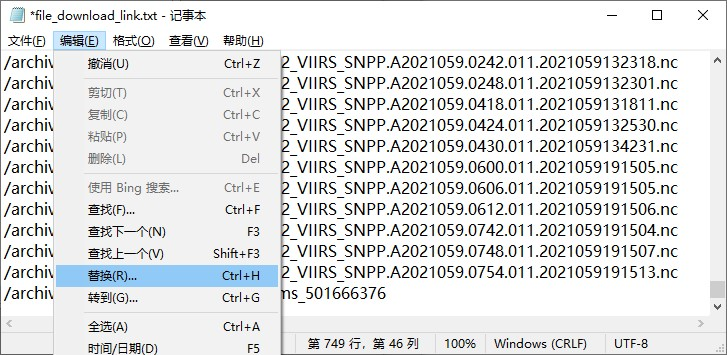
\includegraphics[width=\linewidth]{images/28.替换工具}
\end{frame}
\begin{frame}
    \frametitle{执行替换操作}
    查找内容:/archive\\
    替换为:https://ladsweb.modaps.eosdis.nasa.gov/archive \\
    执行\underline{全部替换},即可达到目的
    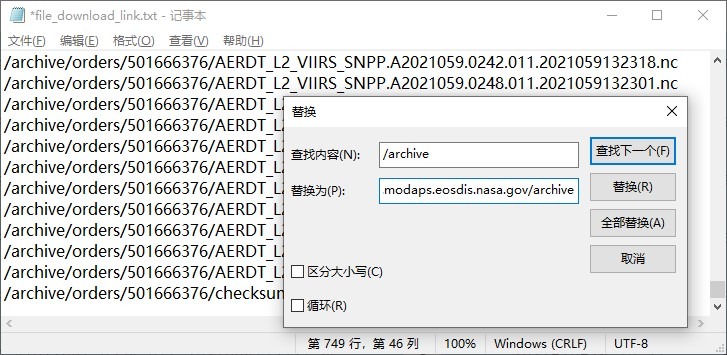
\includegraphics[width=\linewidth]{images/29.替换项目}
\end{frame}
\begin{frame}
    \frametitle{替换结果}
    这样我们就得到了订单中所有文件的真实下载地址
    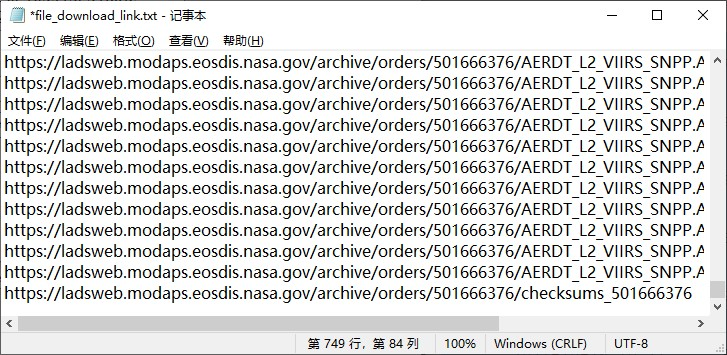
\includegraphics[width=\linewidth]{images/30.替换结果}
\end{frame}
\begin{frame}
    \frametitle{保存文件下载地址}
    将文件保存以备后续下载使用
    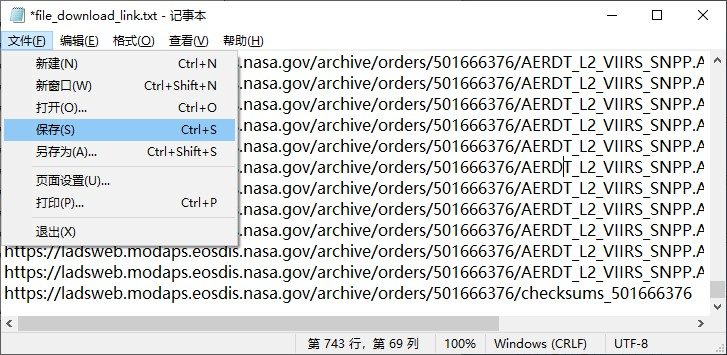
\includegraphics[width=\linewidth]{images/31.保存替换结果}
\end{frame}
\subsection{安装下载工具}
\begin{frame}
    \frametitle{下载Aria2}
    为了加快下载速度,我们使用著名的多线程下载工具Aria2\\
    直接从Aria2在GitHub的仓库下载,以64位1.36.0版为例\\
    \url{https://github.com/aria2/aria2/releases}
    \begin{annotationimage}{width=\linewidth}{images/d_by_aria2/下载Aria2}
        \draw[red,very thick] (0.06,0.54) rectangle (0.32,0.60);
    \end{annotationimage}
\end{frame}
\begin{frame}
    \frametitle{提取Aria2}
    在资源管理器中双击打开下载的压缩包\\
    复制其中的aria2c.exe应用程序
    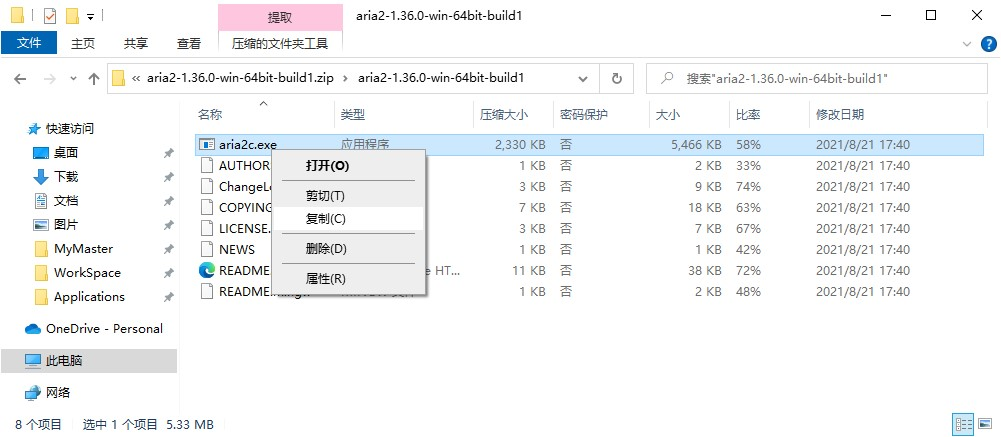
\includegraphics[width=\linewidth]{images/d_by_aria2/打开压缩包}
\end{frame}
\begin{frame}
    \frametitle{放置Aria2程序}
    粘贴到C:\textbackslash Windows\textbackslash System32目录下\\
    以便可以直接在终端窗口访问
    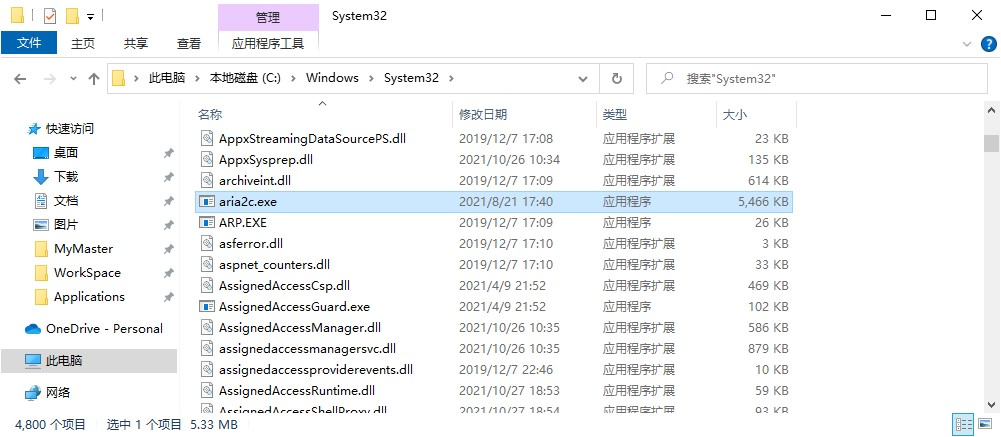
\includegraphics[width=\linewidth]{images/d_by_aria2/放置aria2}
\end{frame}
\subsection{下载}
\begin{frame}
    \frametitle{打开命令窗口}
    按住Shift键,右键订单文件夹空白处\\
    点击\underline{在此处打开Powershell窗口}\\
    在Win7中是点击\underline{在此处打开命令窗口}
    \begin{figure}
        \begin{annotationimage}{width=0.8\linewidth}{images/d_by_aria2/打开Pwershell}
            \draw[red,very thick] (0.3,0.22) rectangle (0.5,0.26);
        \end{annotationimage}
    \end{figure}
\end{frame}
\begin{frame}[label=aria2-cmd]
    \frametitle{下载命令}
    输入下载指令:\\
    aria2c.exe --http-use=登录laads的用户名 --http-passw=登录laadsd的密码
    --continue=true --retry-wait=2 -x 6 -i 存放下载地址的文件名 \\
    不要复制本页命令,请阁下按照自己的实际情况打进去
    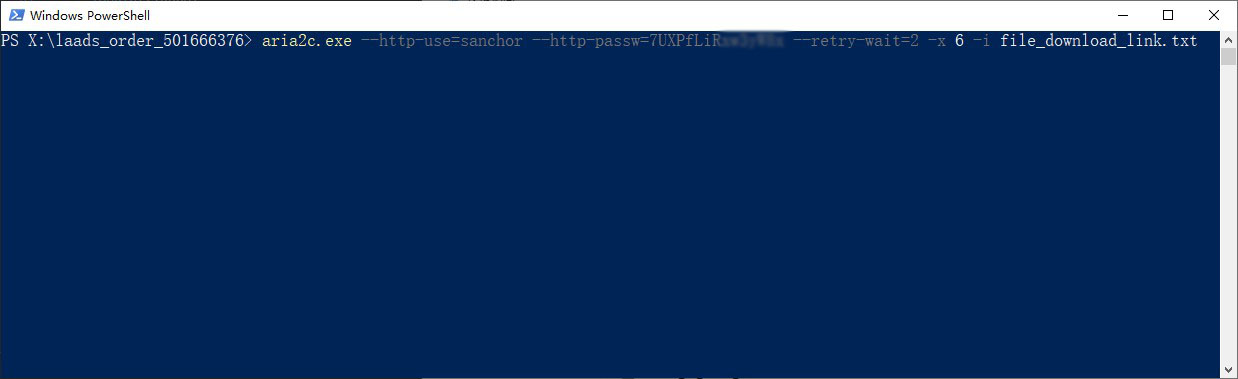
\includegraphics[width=\linewidth]{images/d_by_aria2/下载命令.jpg}
\end{frame}
\begin{frame}
    \frametitle{开始下载}
    输入完命令,敲击回车键开始下载\\
    不出意外你会看到与下图类似的内容,说明正在下载中\\
    即使你不小心关闭了命令窗口,可以再按照上面两张片子重新操作,已下载的文件会被跳过
    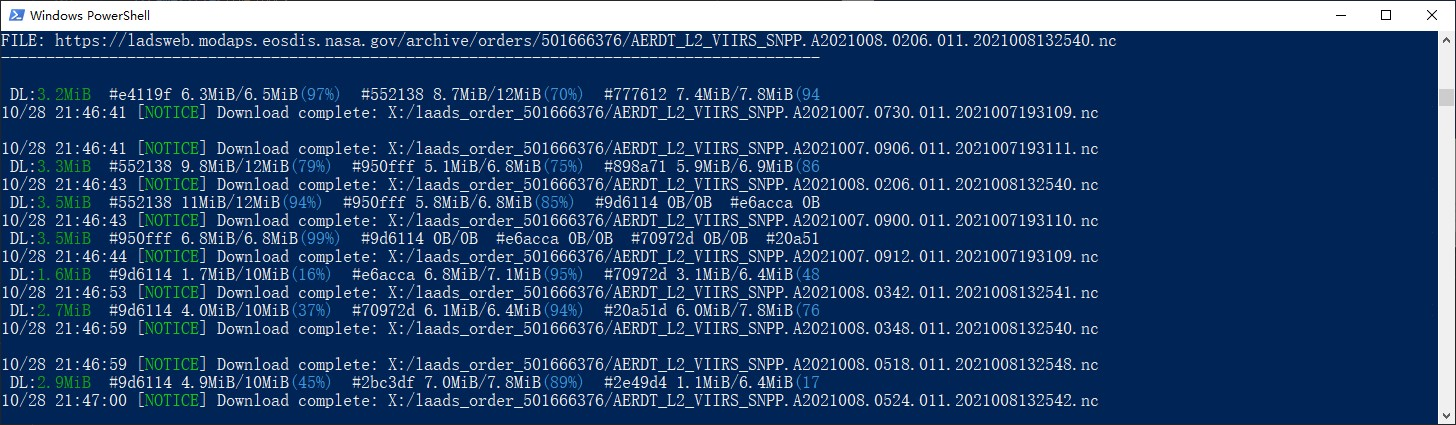
\includegraphics[width=\linewidth]{images/d_by_aria2/开始下载}
\end{frame}
\begin{frame}
    \frametitle{下载完成}
    下载完成时就类似于下图\\
    根据笔者某次下载记录,下载一个21.6G的订单,耗时为2个小时整
    \footnote{订单大小可以在
    \hyperlink{file-link}{\beamergotobutton{获取选中文件地址}}这张片子中查看}
    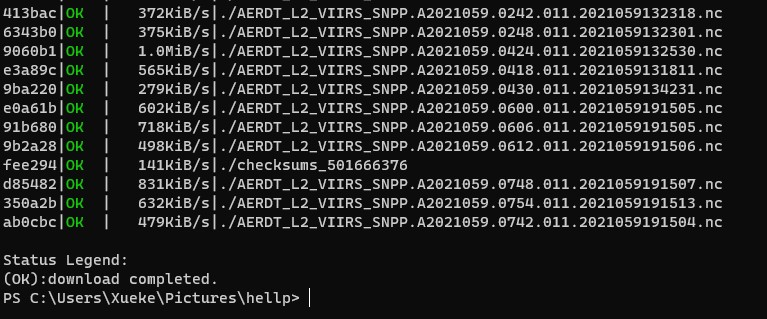
\includegraphics[width=\linewidth]{images/d_by_aria2/下载完成.jpg}
\end{frame}